\section{RIOT}
\label{sec:riot}

\begin{figure}[!ht]
	\centering
	
\includegraphics[width=0.4\textwidth]{./images/chapter4/riot.png}
	\caption[Λειτουργικό σύστημα RIOT.]{Λειτουργικό σύστημα RIOT.\footnotemark}
	\label{fig:riot}
\end{figure}

\footnotetext{\url{https://www.riot-os.org/}}

Το \textit{RIOT} \cite{bib:riot} είναι ένα λειτουργικό σύστημα βασισμένο σε μικροπυρήνα ανοιχτού κώδικα, σχεδιασμένο για να ανταποκρίνεται στις απαιτήσεις των συσκευών IoT και άλλων ενσωματωμένων συσκευών. Αυτές οι απαιτήσεις περιλαμβάνουν ένα πολύ χαμηλό αποτύπωμα μνήμης (της τάξης των λίγων kilobytes), υψηλή ενεργειακή απόδοση, δυνατότητες σε πραγματικό χρόνο, υποστήριξη για ένα ευρύ φάσμα υλικού χαμηλής κατανάλωσης ενέργειας, στοίβες επικοινωνίας για ασύρματα και ενσύρματα δίκτυα.

Το RIOT παρέχει έναν μικροπυρήνα, πολλαπλές στοίβες δικτύου και βοηθητικά προγράμματα που περιλαμβάνουν κρυπτογραφικές βιβλιοθήκες, δομές δεδομένων, ένα τερματικό και άλλα. Το RIOT υποστηρίζει ένα ευρύ φάσμα αρχιτεκτονικών μικροελεγκτών, αισθητήρων και διαμορφώσεων για ολόκληρες πλατφόρμες, π.χ. Atmel SAM R21 Xplained Pro, Zolertia Z1, STM32 Discovery Boards κ.λ.π. σε όλο το υποστηριζόμενο υλικό (πλατφόρμες 32-bit, 16-bit και 8-bit). Το RIOT παρέχει τη δυνατότητα για προγραμματισμό εφαρμογών σε ANSI C και C++, με multireadreading, χρονοδιακόπτες, κ.α.

\noindent Οι κύριοι στόχοι που οδήγησαν στη δημιουργία του RIOT ήταν οι ακόλουθοι:

\begin{enumerate}
	\item Ελαχιστοποίηση χρήσης πόρων μνήμης (RAM/ROM) και κατανάλωσης ενέργειας.
	\item Υποστήριξη για ευέλικτες διαμορφώσεις (από 8-bit έως και 32-bit μικροελεγκτές).
	\item Ελαχιστοποίηση των διπλότυπων κώδικα.
	\item Φορητότητα του μεγαλύτερου μέρους του κώδικα κατά μήκους όλου του υποστηριζόμενου υλικού.
	\item Παροχή μιας πλατφόρμας λογισμικού εύκολης στη χρήση με δυνατότητες πραγματικού χρόνου.
\end{enumerate}

\subsection*{Δομή του λογισμικού}
\label{subsec:structure}

Το RIOT είναι δομημένο σε επιμέρους \textit{ενότητες} (\textit{modules}) λογισμικού οι οποίες είναι συγκεντρωμένες γύρω από έναν πυρήνα που προσφέρει μινιμαλιστική λειτουργικότητα \cite{bib:riot_new}. Κατ' αυτόν τον τρόπο παρέχεται η δυνατότητα για την κατασκευή ενός ολοκληρωμένου συστήματος, συμπεριλαμβάνοντας μόνο τις ενότητες που είναι απαραίτητες για την εκάστοτε \textit{περίπτωση-χρήσης} (\textit{use-case}), ελλατώνοντας έτσι στο ελάχιστο την κατανάλωση μνήμης και γενικότερα την πολυπλοκότητα του συστήματος.

Σε ένα υψηλότερο επίπεδο, ο πηγαίος κώδικας του RIOT είναι δομημένος σύμφωνα με τις ακόλουθες ομάδες (groups), όπως φαίνεται και στο \autoref{fig:riot_struct} \cite{bib:riot_new}:

\begin{itemize}
	\item \textbf{core:} Υλοποιεί τον πυρήνα και τις βασικές δομές δεδομένων του.
	\item \textbf{Αφαίρεση υλικού}
	\begin{itemize}
		\item cpu: Υλοποιεί όλες τις λειτουργίες του μικροελεγκτή που χρησιμοποιείται. Αυτές μπορεί να είναι κώδικας για τον χειρισμό των διακοπών (interrupts), του ρολογιού (clock) συστήματος, των χρονοδιακοπτών και των προγραμμάτων οδήγησης για περιφερειακά όπως είναι τα UART και SPI.
		\item boards: Επιλέγει, διαμορφώνει και καθορίζει τις κύριες μονάδες επεξεργασίας (CPU) και τα προγράμματα οδήγησης (drivers) που χρησιμοποιούνται.
		\item drivers: Υλοποιεί τα προγράμματα οδήγησης των συσκευών. Κατά κανόνα, ελέγχει εξαρτήματα συνδεδεμένα στην CPU μέσω ακροδεκτών γενικού σκοπού (GPIO) και διαύλων όπως I2C, SPI ή UART.
		\item periph: Παρέχει ενοποιημένη πρόσβαση στα περιφερειακά των μικροελεγκτών και χρησιμοποιείται από τα προγράμματα οδήγησης των συσκευών.
	\end{itemize}
	\item \textbf{sys:} Υλοποιεί βιβλιοθήκες πέραν των λειτουργιών του πυρήνα.
	\item \textbf{pkg:} Εισάγει εξαρτήματα από τρίτους.
	\item \textbf{application:} Υλοποιεί την υψηλού-επιπέδου λογική της πραγματικής use-case.
\end{itemize}

\begin{figure}[!ht]
	\centering
	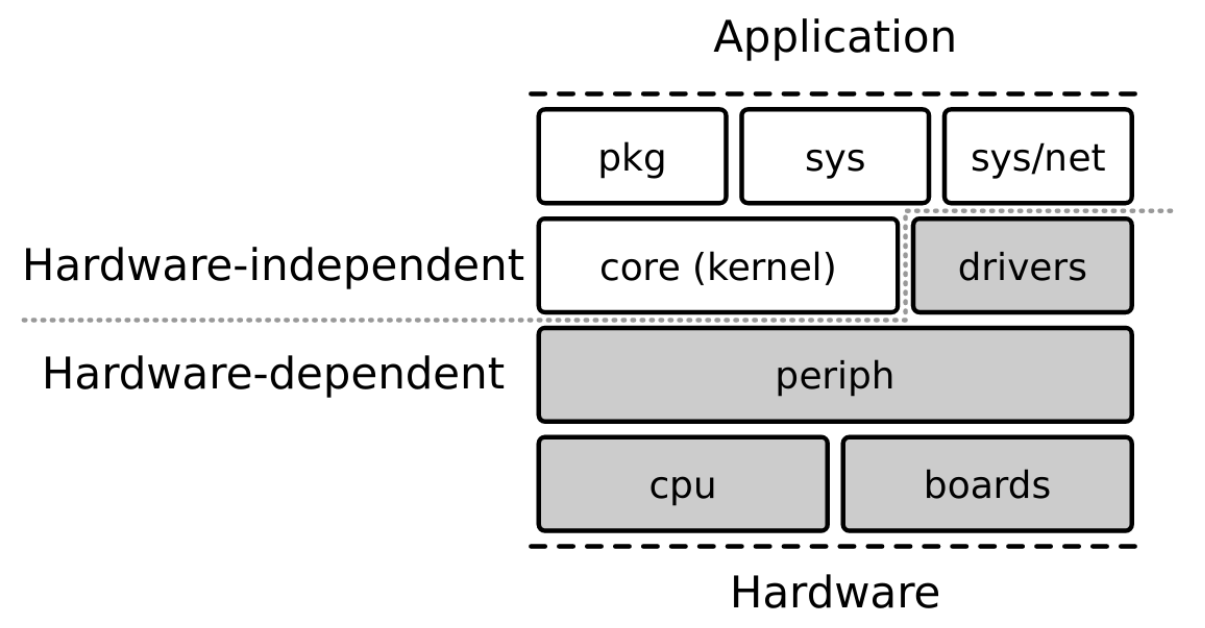
\includegraphics[width=0.6\textwidth]{./images/chapter4/riot_struct.png}
	\caption[Λειτουργικό σύστημα RIOT.]{Δομικά στοιχεία του RIOT.}
	\label{fig:riot_struct}
\end{figure}